\ifdefined\included
\else
\setcounter{chapter}{0}
\dominitoc
\faketableofcontents
\fi

\chapter{Human-Robot Collaboration Context}
\chaptermark{Human-Robot Collaboration Context}
\label{chap:1}
\minitoc

%%%%%%%%%%%%%%%%%%%%%%%%%%%%%%%%%%%%%%%%%%%%%%%%%%%%%%%%%%%%%%%%%%%%%%%%%%%%%%%%%%%%%%

\chapabstract{This chapter provides more details about the context of my PhD by discussing related fields and works of \acrshort{hrc}. This chapter eventually highlights the gap in the literature that motivates my PhD work.}

%%%%%%%%%%%%%%%%%%%%%%%%%%%%%%%%%%%%%%%%%%%%%%%%%%%%%%%%%%%%%%%%%%%%%%%%%%%%%%%%%%%%%%

\section{Multidisciplinarity of Human-Robot Interaction}

\begin{figure}
    \center
    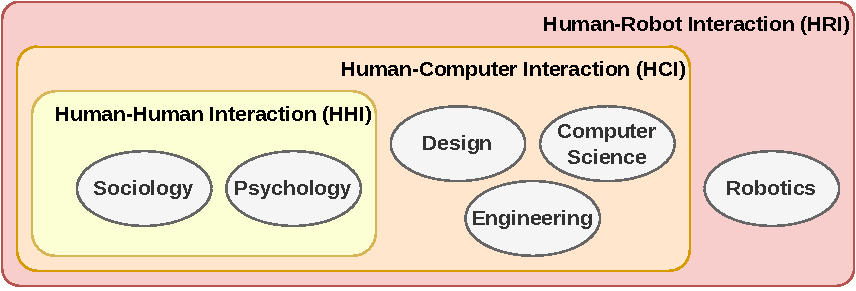
\includegraphics[width=\linewidth]{Chapter1/hri_multi.pdf}
    \caption{Multidisciplinarity of the Human-Robot Interaction field.}
    \label{fig:hri_multi}
\end{figure}

In \cite{bartneck_human_robot_2020}, the \acrfull{hri} is considered unique because of the interaction of humans with social robots, which is at the core of this multidisciplinary research field. These interactions usually include physically embodied robots, and their embodiment makes them inherently different from other computing technologies. Moreover, social robots are perceived as social actors bearing cultural meaning, strongly impacting contemporary and future societies. Saying that a robot is embodied does not mean it is simply a computer on legs or wheels. Instead, we must understand how to design that embodiment, both in terms of software and hardware, as it is commonplace in robotics, and in terms of its effects on people and the kinds of interactions they can have with such a robot.

Overall, \acrfull{hri} focuses on developing robots that can interact with people in various everyday environments. This opens up technical challenges resulting from the dynamics and complexities of humans and the social environment. This also opens up design challenges—related to robotic appearance, behavior, and sensing capabilities—to inspire and guide interaction. From a psychological perspective, \acrshort{hri} offers the unique opportunity to study human affect, cognition, and behavior when confronted with social agents other than humans. In this context, social robots can be research tools to study psychological mechanisms and theories.

As a result, by taking inspiration from \acrfull{hhi} and \acrfull{hci}, \acrshort{hri} is an endeavor that brings together ideas from a wide range of disciplines such as Engineering, Computer Science, Robotics, Psychology, Sociology, and Design.
In the following, we discuss some related aspects and works of the mentioned disciplines by categorizing them between \acrshort{hhi}, \acrshort{hci}, and \acrshort{hri} as depicted in figure~\ref{fig:hri_multi}.

\subsection{Human-Human Interaction}

Many works dealing with interacting with humans take inspiration from \acrfull{hhi}, including research in sociology and psychology. \acrshort{hhi} refers to the communication and collaboration between two or more individuals, where humans engage in various forms of social, cognitive, and emotional exchanges. Such interaction can occur through verbal and non-verbal communication, such as speech, gestures, facial expressions, and body language.   

Since communication has a crucial role in collaboration, communication theories have been widely studied for a long time \cite{cherry_human_1957,smith_designing_1998}. Professor Albert Meharbian indicates in \cite{mehrabian1967decoding} that, when communicating feelings, the words pronounced, the voice tone, and the body language correspond respectively to 7\%, 38\%, and 55\% of the effective communication. These results suggest that communication, especially about feelings, is more complex than ``simply'' finding the right words. The way these words are pronounced and shared strongly affects the message sent. The Grice's four maxims of conversation \cite{grice1975logic}, or Gricean maxims, can also be mentioned and describe the relevance of four distinct aspects of communication: quantity, quality, relation, and manner. These four maxims describe specific rational principles observed by people who follow the cooperative principle in pursuit of effective communication.

\acrshort{hhi} also led to studies on collaboration, teamwork, and so-called Joint Action theories \cite{cohen_team_1970,levesque_acting_1990,cohen_teamwork_1991}. As put in \cite{sebanz_2006joint}, these works aim to describe and understand social interaction whereby two or more individuals coordinate their actions in space and time to bring about a change in the environment, usually trying to reach a common goal.

We must first understand how humans interact with each other before making robots able to interact correctly with humans. However, perfectly mimicking humans is questionable since robots fundamentally differ from humans. Humans have created robots to help and assist them. Thus, HHI should inspire robot design, but additional research is mandatory to determine how to create appropriate interactive and collaborative robots.

\subsection{Human-Computer Interaction}

A first step of artificial interaction and collaboration is the field of \acrfull{hci}. \acrshort{hci} is the field of study that focuses on optimizing how users and computers interact by designing interactive computer interfaces that satisfy users' needs. It is a multidisciplinary subject covering computer science, behavioral sciences, cognitive science, ergonomics, psychology, and design principles.
Today, \acrshort{hci} focuses on designing, implementing, and evaluating interactive interfaces that enhance user experience using computing devices. This includes user interface design, user-centered design, and user experience design. 

This field is made up of four key components: 
The User, along with their needs, goals, interaction patterns, cognitive capabilities, emotions, and experiences; 
The Goal-Oriented Task which is the objective or goal the user has in mind; 
The Interface is about the overall user interaction experience through senses such as touch, click, gesture, voice, display size, and colors;
The Context must be taken into account because it influences the interaction. 

To produce easy interaction with robots, the study of \acrshort{hci} is relevant and helps to design intuitive, user-friendly interactive robots.

\subsection{Human-Robot Interaction}

\acrfull{hri} is a field of study exploring the design, development, and evaluation of robots interacting with humans in various settings. \acrshort{hri} aims to create robots that can effectively and seamlessly collaborate with humans in domestic environments, workplaces, or other contexts. 
\acrshort{hri} can be categorized in several domains, not necessarily exclusive. Here are some examples:

\uline{Social robotics} focuses on social interactions with humans and, thus, explores how robots can understand and respond to human emotions, social cues, and communication styles.
A significant amount of work is dedicated to \acrshort{hri} in Healthcare to assist patients, especially the elderly and children with conditions. Those works are also usually linked to emotion-aware robotics focused on recognizing and responding to human emotions using affective computing techniques. A common application is storytelling for children to convey ideas, feelings, or culture. 

\uline{Human-Centered Robotics} emphasizes the importance of considering human needs and preferences. This subfield often involves user studies to ensure and identify if and how robots are user-friendly and can seamlessly integrate into human environments.

\uline{Robot Ethics} is another central subfield focused on considerations such as privacy, safety, responsibility/accountability, and the impact of robots on society.

\uline{Explainable AI and transparency} are a growing interest in making decision-making processes more understandable to humans, and thus, help robots be legible, predictable, and acceptable.

\uline{Computational \acrshort{hri}}, as described in~\cite{thomaz_computational_2016}, is the subset of \acrshort{hri} concerned explicitly with the algorithms, techniques, models, and frameworks necessary to build robotic systems that engage in social interactions with humans. This thesis is part of this category because it is focused on developing task planning algorithms and models relevant to a collaborative robot. 

\uline{Human-Robot Collaboration} or \uline{Collaborative Robotics} focuses on developing robots that work alongside humans in shared workspaces, usually as a team. \acrshort{hrc} is the main topic of my thesis and is a vast subject worth delving into. Hence, the following section is dedicated to providing more details about \acrshort{hrc}.

%%%%%%%%%%%%%%%%%%%%%%%%%%%%%%%%%%%%%%%%%%%%%%%%%%%%%%%%%%%%%%%%%%%%%%%%%%%%%%%%%%%%%%
\section{Human-Robot Collaboration}

\acrfull{hrc} refers to the synergy and cooperation between humans and robots in shared environments to achieve common goals. In \acrshort{hrc}, humans and robots work together, often leveraging their complementary strengths to enhance overall performance and efficiency. According to human desires, the robot can also act in a way that eases and facilitates the human part of the task. This collaborative approach involves close interaction, communication, and coordination between human and robotic agents.

\subsection{Inspirations \& Theories informing HRC}

This interdisciplinary field takes inspiration from various theories and fields, as introduced earlier. Nevertheless, three main inspirations can be highlighted:

\subsubsection*{Belief Desire Intention Model:} The belief-desire-intention (BDI) model was originally developed by Michael Bratman~\cite{Bratman1987_BRAIPA}. This model is used in intelligent agents research to describe and model intelligent agents. Straightforwardly, the BDI model is characterized by the implementation of the three notions appearing in its name, i.e., an agent's beliefs (knowledge of the world from the perspective of the agent), desires (objective or goal to accomplish), and intentions (the planned course of actions to achieve the agent's desire). 

\subsubsection*{Shared Cooperative Activity:} Shared cooperative Activity defines prerequisites for an activity to be considered shared and cooperative. The main ones are mutual responsiveness, commitment to the joint activity, and commitment to mutual support. A good example to clarify these prerequisites is a scenario where agents move a table together. Mutual responsiveness ensures that the agents' movements are synchronized. The commitment to the joint activity reassures each agent that the others will not drop their side and quit the joint activity. Finally, the commitment to mutual support deals with possible breakdowns due to one agent's inability to perform part of the plan.  

\subsubsection*{Joint Intention \& Action Theory:} 
Joint Intention Theory proposes that for joint action to emerge, team members must communicate to maintain a set of shared beliefs and to coordinate their actions toward the shared plan~\cite{cohen_teamwork_1991}. In collaborative work, agents should be able to count on the commitment of other members. Therefore, each agent should inform the others when they conclude that a goal is achievable, impossible, or irrelevant~\cite{hoffman2004collaboration}.

\subsection{Key Aspects}

% More concretely, some key aspects of a seamless collaboration are listed and commented on below to better picture what the theories above involve in practice. 

In order to better picture the implications of the above theories, some key aspects of a seamless collaboration are listed and commented on below. This list is not exhaustive, but it highlights some skills that humans naturally exhibit and that a robot must be endowed with to collaborate with them. 

\textbf{Specialization of Roles:} There are several human-robot relationships, including supervisor-subordinate, partner-partner, teacher-learner, and leader-follower. These roles can be predefined and fixed during the whole collaboration. The role distribution can also be flexible using weighting functions that allow a continuous change between the roles to adapt to every context and situation.

\textbf{Establishing shared goal(s):} Through direct discussion or inference, agents must determine and agree on the shared goals they are trying to achieve. However, a shared goal is not always necessary and can be established in the middle of a task execution either by the human or the robot.

\textbf{Allocation of subtasks:} After deciding how to achieve their goals, agents must determine what actions and subtasks will be done by each agent and how to coordinate each other. This can be done explicitly before starting the task or reactively done on the fly.

\textbf{Progression tracking:} Agents must be able to track progress toward their goals. That is, they must be able to determine what has been achieved, by whom, and what remains to be done. 

\textbf{Communication:} Any collaboration requires communication, verbal or not. Most of the mentioned aspects can or must involve communication. However, it is essential to identify what and how to communicate during the collaboration. Communicating too much can be annoying, while not enough can induce confusion and harm collaboration.

\textbf{Adaption and learning:} On a short-term scale, agents must adapt to each other and the environment. In the longer term, agents must also learn from other partners and the acquired experience.

\textbf{Ergonomics:} It should be intuitive to collaborate and communicate with the robot. This aspect must be considered when designing the robot's hardware and software. Ergonomics is a central aspect of Human-Computer Interaction. Thus, many works from this field can be used in our context or serve as inspiration.

\textbf{Explainability:} This aspect is important for seamless collaboration as the human should be able to understand what the robot is doing and why. This topic is getting more and more attention and is often referred to as Explainable AI. This is especially relevant to counter the \textit{black box} tendency of machine learning where it's impossible to explain a specific decision. Being explainable often enhances predictability, which is also essential for a collaborative robot.

\subsection{Architectures \& Complete Systems}

It is important to remember that since a collaborative robot is issued from an interdisciplinary field, its different functionalities and capabilities are usually separated into several dedicated components. These components interact and communicate with each other, forming a complete architecture. Such architectures cover all aspects relevant to exhibiting the robot's behavior, from sensory perception to physical motions, including reasoning processes. 
Despite developing distinct robotic components, the robot must be considered a whole. Each component cannot be studied entirely independently of other aspects of the complete system. As a result, optimizing how these components interact by design has been the focus of several works proposing robotic architectures.

\begin{figure}
    \center
    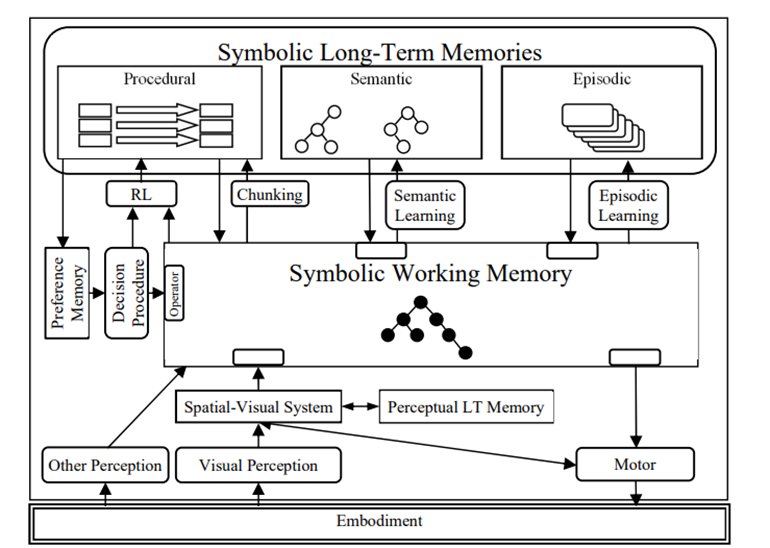
\includegraphics[width=0.9\linewidth]{Chapter1/soar_architecture.png}
    \caption{The SOAR cognitive architecture.}
    \label{fig:soar}
\end{figure}

As Matthias Scheutz, Jack Harris, and Paul Schermerhorn put in \cite{scheutz_systematic_2013}, architectures for intelligent robots have improved steadily over the years. 
Early works like \cite{alami_designing_1993,alami_architecture_1998,chatila_integrated_1992} propose architectures to provide autonomy to mobile robots, focusing on three levels: decision, execution, and functional. Diverse components that allow robots to negotiate increasingly more complex indoor and outdoor environments have been considered, and they have improved those architectures over the years. As a result, current robot architectures integrate multiple sophisticated algorithms for real-time perceptual, planning, and action processing, from 3D object recognition to simultaneous localization and mapping to navigation and task planning to action sequencing. However, classical robotic architectures like the ones mentioned above typically lack components for high-level cognition, such as general-purpose reasoning and problem-solving. 
To address this issue, studies on cognitive robot architecture began mainly with the SOAR (depicted in figure~\ref{fig:soar}) and ACT-R architectures \cite{laird_soar_1987,anderson2004integrated}.
Often based on the structure of the human mind, such cognitive architectures aim to endow robots with high-level capabilities like learning, inferring, and reasoning about how to behave in response to complex goals in complex worlds. 

\cite{lemaignan_artificial_2017} identifies relevant collaborative cognitive skills and integrates them into a proposed architecture. The skills include geometric reasoning and situation assessment based on perspective-taking and affordance analysis; acquisition and representation of knowledge models for multiple agents (humans and robots, with their specificities); situated, natural, and multi-modal dialogue; human-aware task planning; human-robot joint task achievement.

\cite{thierauf_toward_2024} proposes another integrated cognitive robotic architecture more focused on self-awareness. It allows the robot to assess its own performance, identify task execution failures, communicate them to the humans, and resolve them, if possible. 



%%%%%%%%%%%%%%%%%%%%%%%%%%%%%%%%%%%%%%%%%%%%%%%%%%%%%%%%%%%%%%%%%%%%%%%%%%%%%%%%%%%%%%
\section{Models for Interaction}


A robotic agent interacting with a human must coordinate its actions with them. Moreover, joint action theory exhibits that humans interacting together represent the task as a whole and plan not only for their actions but also for the actions of other agents. Thus, we think that for a human to perform the most efficient and satisfactory joint task with a robot, this robot must explicitly model human actions and plan not only for its actions but also for the human ones. This is why we present in this section some notations to clarify the different models used in this thesis, and then we present in more detail how to model tasks.

\subsection{Human and Robot Agents}

\begin{figure}
    \centering
    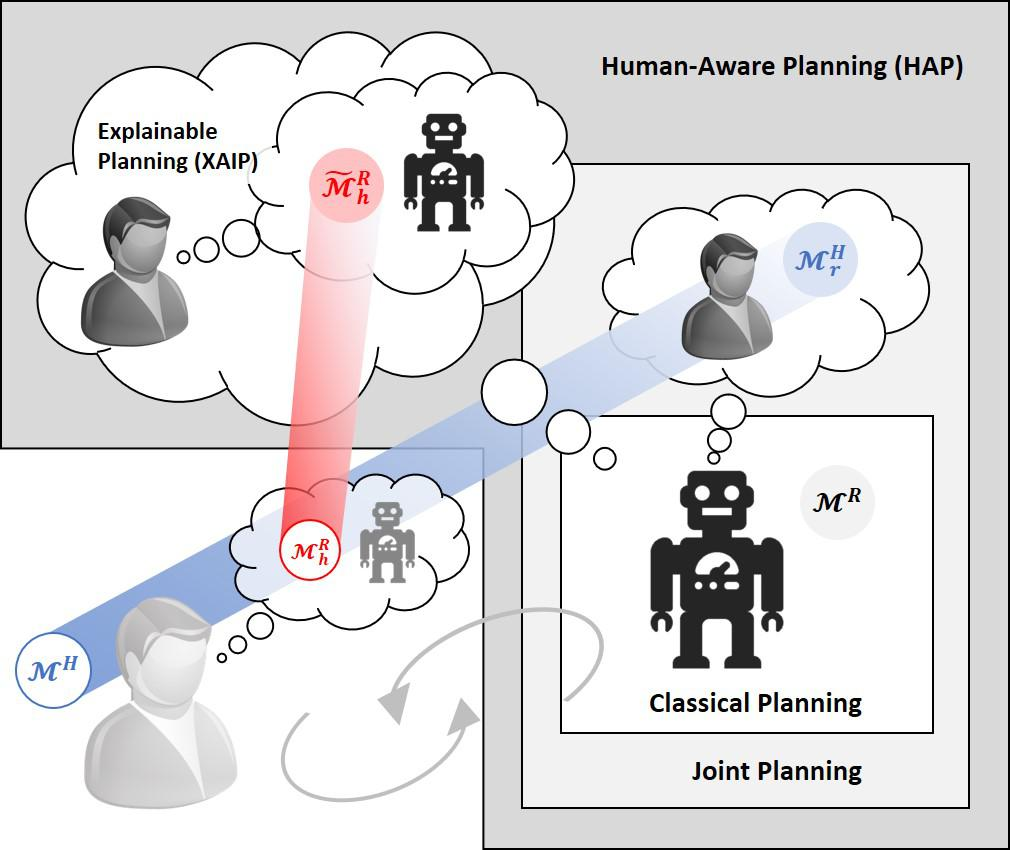
\includegraphics[width=0.8\linewidth]{Chapter1/chakraborti_notations.jpg}
    \caption{Agent models from Chakraborti \textit{et al.} notations.}
    \label{fig:chakraborti_notations}
\end{figure}

Chakraborti \textit{et al.} introduced notations to differentiate between the models used in this thesis in their work~\cite{ChakrabortiBTZS15}, also used in Buisan's thesis~\cite{thesisBuisan21}. These notations summarize and differentiate elegantly the different models manipulated in the \acrshort{hri}/\acrshort{hrc} field. These notations are depicted in figure~\ref{fig:chakraborti_notations}. At the bottom are depicted the human agent (on the left) and the robot agent (on the right). When solving a task alone, the robot uses its own model referred to as $\mathcal{M}^R$. This case can be considered as a Classical Planning problem. 
Then, $\mathcal{M}^H_r$ is an estimation by the robot of the model of the human. Finally, $\tilde{\mathcal{M}}^R_h$ is an estimation of the robot model the human has. These models are likely to include knowledge about the world from the agent's perspective, an action model describing the agent's capabilities, and an agenda capturing the goal and motivation of the agent.

It is important to remember that when discussing a task planner, it is considered part of the robot. Thus, $\mathcal{M}^R$ is the robot's ground truth. As a consequence, if there is a belief divergence between $\mathcal{M}^H_r$ and $\mathcal{M}^R$, we always consider that $\mathcal{M}^R$ is the truth. Otherwise, it would make no sense to keep this information in $\mathcal{M}^R$ while having access to the one in $\mathcal{M}^H_r$.

\subsection{Task Modeling}

A common way of representing human activity ($\mathcal{M}^H_r$) and interaction with computers at a high abstraction level is by using task models. The hierarchical structure of human activity was first exploited by Annett and Duncan \cite{annett1967task}. They state that tasks can be described at several levels of abstraction until a certain criterion is met. Each task can thus be refined into subtasks detailing the procedure the human follows to achieve the higher level task. Task modeling has then evolved to introduce interaction with systems, produced and needed information, potential errors, and a wide variety of operator specifying how tasks interact with each other during their execution. Task models are now commonly used in user-centered and user-interface design processes. Most advanced notations include ConcurTaskTrees \cite{paterno2004concurtasktrees} and HAMSTERS \cite{martinie2019analysing}. These models are used to design or evaluate interactive systems. They allow the designer to understand the user task better or to study the user workflow using their system. However, these models contain too little information for a system to be able to reason and make decisions on them (either in planning or acting).


\subsection{Hierarchical Models}

In classical planning, each action of an agent is atomic and needs some conditions to hold in the environment to be executed, and then it changes the environment when applied. The planning process then has to find the right sequence of actions, applicable one after the other, to change the environment and reach a specific goal state. 

However, humans tend to work more abstractly and decompose tasks hierarchically into smaller tasks until the action level is reached. In practice, using \acrfull{htn} allows the domain designer to help the plan search by inserting expert knowledge via a hierarchy linking the actions \cite{erol_complexity_1996}. A task network consists of tasks organized in a fully or partially ordered manner, and each task can be either abstract or primitive. Primitive tasks are elementary tasks that can be achieved by performing one associated action.
On the other hand, abstract tasks are tasks that first need to be decomposed into other subtasks, ``more primitive''. The planner's goal is not to find the sequence of actions to reach a goal but to select recursively for each task the suitable decomposition ending (if possible) with a network of actions applicable from the initial state. Ghallab, Nau, and Traverso name such a process as \textit{planning with refinement methods} \cite{ghallab2016automated}. This planning hierarchy allows the domain designer to guide the search by inserting some expertise into the model and enhancing explainability as the decompositions often offer a semantic to their subtasks. The 'why' of a subtask can usually be answered by going up in the hierarchy, while the 'how' is answered by going down. 

\begin{figure}
    \center
    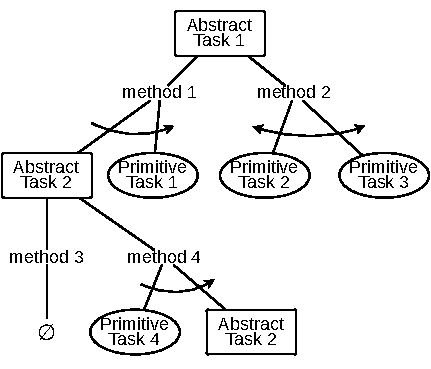
\includegraphics{Chapter1/htn_example.pdf}
    \caption{An HTN example. Rectangles represent abstract tasks. Each method describes a possible way to decompose an abstract task if its preconditions are met. Methods can decompose abstract tasks into primitive tasks (ellipses) and/or into other abstract tasks. The obtained subtasks can be fully ordered, such as with \emph{method 1} (represented with a one-way arrow), or partially ordered, like \emph{method 2} (represented with a two-way arrow). Note that methods can also decompose a task into nothing like \emph{method 3}, for instance, when the task is already done, and they can be recursive like \emph{method 4}.
    }
    \label{fig:htn_example}
\end{figure}

To better picture \acrshort{htn} models, a symbolic example is depicted in figure~\ref{fig:htn_example}.
Rectangles represent abstract tasks. Each method describes a possible way to decompose an abstract task if its preconditions are met. Methods' preconditions are not necessarily mutually exclusive. Hence, as mentioned above, it is the planner's job to select the most suitable one when several ones are applicable.
Methods decompose abstract tasks into primitive tasks, represented with ellipses, and/or into other abstract tasks. The obtained subtasks can be fully ordered, such as with \emph{method 1} (represented with a one-way arrow) where \emph{Abstract Task 2} has to be completed before \emph{Primitive Task 1}. Methods can also be partially ordered as with \emph{method 2} (represented with a two-way arrow) where \emph{Primitive Task 2} and \emph{Primitive Task 3} can be achieved in any order. Note that methods can also decompose a task into nothing like \emph{method 3}, for instance, when the task is already done. Moreover, methods can be recursive like \emph{method 4}.

\begin{figure}
    \center
    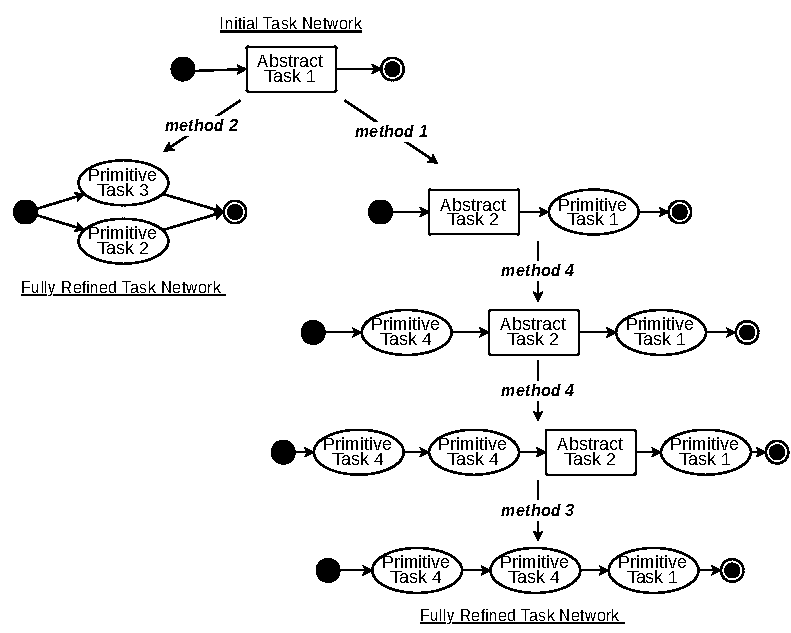
\includegraphics[width=0.9\linewidth]{Chapter1/htn_decomposition_example.pdf}
    \caption{Two possible decompositions of a task network using the HTN described in fig~\ref{fig:htn_example}. Both \emph{method 1} and \emph{method 2} can be applied, leading to two different solutions.
    }
    \label{fig:htn_decomposition_example}
\end{figure}

Now, let us look at an example of a refinement process. We consider an initial task network only composed of \emph{Abstract Task 1}, and we refine it using the HTN described in fig~\ref{fig:htn_example} until the task network only contains primitive tasks (actions). Initially, \emph{method 1} and \emph{method 2} are both applicable and, thus, are candidates to decompose \emph{Abstract Task 1}. Applying \emph{method 2} leads directly to a fully refined solution task network, including two partially ordered primitive tasks (\emph{Primitive Task 2} and \emph{Primitive Task 3}). On the other hand, \emph{method 1} can be applied, leading to a different task network that still includes abstract tasks. Then, \emph{Abstract Task 2} is recursively decomposed using M4 twice. This could correspond to scenarios like filling a box with two balls. Thus, M4 is only applicable until two more balls are in the box. Eventually, only M3 is applicable and refines \emph{Abstract Task 2} into nothing, leading to another solution task network.

%%%%%%%%%%%%%%%%%%%%%%%%%%%%%%%%%%%%%%%%%%%%%%%%%%%%%%%%%%%%%%%%%%%%%%%%%%%%%%%%%%%%%%
\section{Task Planning Overview}

\subsection{Classical Planning}

As Ghallab, Nau, and Traverso put it, “the purpose of planning is to synthesize an organized set of actions to carry out some activity”~\cite{ghallab2016automated}. 
Classical planning is a type of planning that assumes deterministic and fully observable environments. It involves representing the world as a set of states and actions, with plans derived through state space search algorithms. Actions have preconditions and effects, and planning problems entail finding a sequence of actions to transform an initial state into a goal state. Classical planning algorithms, including STRIPS, Graphplan, and Fast Downward, utilize heuristics to guide the search efficiently. While well-suited for domains with precise and deterministic dynamics, classical planning may face challenges in handling uncertainty or partial observability, leading to alternative planning approaches for such scenarios.

\subsection{Task Planning for hrc}

Classical planning has been vastly studied and can now solve various problems efficiently. However, the intricate nature of \acrshort{hrc} scenarios demands sophisticated task planning methodologies capable of adapting to dynamic environments, understanding human intent, and promoting a fluent exchange of information. Hence, several subfields of task planning have emerged and are used in \acrshort{hrc}. Here are a few examples:

\begin{itemize}
    \item \textbf{Hierarchical Task Planning} is a technique that organizes tasks in a hierarchical structure presented in the previous section, allowing for the representation of complex tasks at various abstraction levels. This approach enhances modularity, flexibility, and explainability in task planning, accommodating intricate collaborative scenarios.
    
    \item \textbf{Mixed-Initiative Planning} leverages the strengths of both humans and robots by allowing for a dynamic allocation of decision-making authority. This technique promotes collaborative decision-making, enabling the system to adapt to the expertise and preferences of each agent involved in the collaborative task.
    
    \item \textbf{Human-Centric Task Planning} focuses on incorporating human factors into the planning process. This involves understanding human capabilities, preferences, and cognitive load to optimize task plans that align with human collaborators' natural workflows and expectations.
    
    \item \textbf{Learning-Based Task Planning} has emerged thanks to advancements in machine learning as a frontier in adapting to evolving environments. This technique involves training models to understand patterns in human behavior, enabling the robot to learn and adapt its task planning strategies over time. Such techniques can also be used to predict human behavior and consequently adapt the robot's actions.
    
    \item \textbf{Probabilistic Task Planning} integrates uncertainty into the planning process, acknowledging the inherent unpredictability of human behavior and environmental factors. By incorporating probabilistic models, this technique enhances the robustness of task plans in dynamic and uncertain collaborative settings.
    
    \item \textbf{Task and Motion Planning} combines symbolic and geometric reasoning to plan agents' actions. In our context, it can be helpful to consider safety spatial areas near humans and adapt both the robot's motion and decisions. 
    
\end{itemize}

Overall, \textbf{Human-Aware Task Planning} is the process of considering the presence and behavior of humans in the planning and execution of robot tasks. It involves taking into account cues from the shared environment and the dynamics of human-robot interaction. The goal is to generate robot policies that are adaptable, robust, and efficient in crowded and dynamic environments. A detailed presentation and discussion about existing task planning works for \acrshort{hrc} is provided in the related work section (\ref{sec:ch2_related_work}) of Chapter~\ref{chap:2}.  

\subsection{Other Use Cases}

Despite being designed for Human-Robot Collaboration, the task planning techniques presented in this work can be used in other interactive contexts. 

For instance, instead of planning robot actions, we could plan verbal answers in a dialogue. 
This approach is used in \cite{de_carolis_verbal_2000} and \cite{de_carolis_behavior_2001}.
Hence, some algorithms and models proposed in this manuscript could be used to anticipate the possible human sentences and plan the relevant robot communications. 

Additionally, one could think about a smart environment, e.g., a domotic house, where various sensors and actuators are connected. When humans explore and operate in such an environment, it could be relevant to plan domotic actions according to human behavior, e.g., proactively making coffee, opening stores, activating the robot vacuum cleaner, etc. This context is addressed in \cite{pecora_constraint_based_2012} to provide proactive human support.


%%%%%%%%%%%%%%%%%%%%%%%%%%%%%%%%%%%%%%%%%%%%%%%%%%%%%%%%%%%%%%%%%%%%%%%%%%%%%%%%%%%%%%
\section{Human-Aware Navigation}

In my work, I studied the decision-making challenge, mainly in the field of task planning. 
Nevertheless, I also worked on decision-making processes for navigation, more precisely, on how to simulate a navigating interactive human agent endowed with decisional capabilities to challenge robotic navigation systems. Hence, to better understand this contribution, this section provides some context on robot navigation, especially on state-of-the-art techniques and existing benchmarking tools.

As stated in \cite{thesisBuisan21}, robot navigation aims to make the robot base (the whole robot) move from one place to another while avoiding static and moving obstacles. However, other constraints must be added when the robot has to move in an environment where humans are evolving. 
Humans should not just be avoided as other moving obstacles, and their psychological and mental state must be taken into account. Hence, the robot should neither move threateningly, block the humans, nor induce drastic changes in their motion. Taking all these aspects into account is what is called human-aware robot navigation.

\subsection{Robot Navigation techniques}

State-of-the-art techniques for robot navigation involve two kinds of motion planners: a global and a local planner. The global planner is in charge of finding the best overall trajectory to lead the robot to its goal and producing a global plan. This planner usually only takes into account static obstacles described by a given map of the environment. Then, the local planner is responsible for producing velocity commands sent to the motor controllers to follow the produced global plan. To produce the velocity commands, the local planner may produce a local plan with only a few seconds of time horizon that follows the global plan while considering obstacles detected in real-time by the robot sensors, including moving obstacles. This way, the robot should reach its goal while reacting to moving obstacles. 

However, as explained above, such approaches are insufficient in human-populated environments. Humans must be detected and treated differently during the motion planning process. Human-aware approaches detect and track nearby humans and try to estimate their trajectory to plan the robot's one accordingly. This is achieved in works like \cite{singamaneni2021human}, where the human trajectory is estimated using goal recognition processes and elastic bands methods. Then, the robot's motion is planned using tuned elastic band methods to account for the robot's goal, the estimated human trajectory, and other social norms.   

\subsection{Benchmarking tools and metrics}

Where it is easy to benchmark robot navigation on objective metrics like the time to reach a goal, the distance traveled, and the number of collisions \cite{perille2020benchmarking}, it is more challenging to benchmark their human-aware properties.
First, there is no consensus on the metrics to evaluate a navigation system's human-aware properties. State-of-the-art metrics involve proxemics \cite{samarakoon2022review}. However, other relevant metrics, such as the deviation imposed on human motion and the feeling of threat produced, can be used.
Also, finding a usable system that will effectively challenge a \acrfull{han} system is challenging. 

\begin{figure}
    \center
    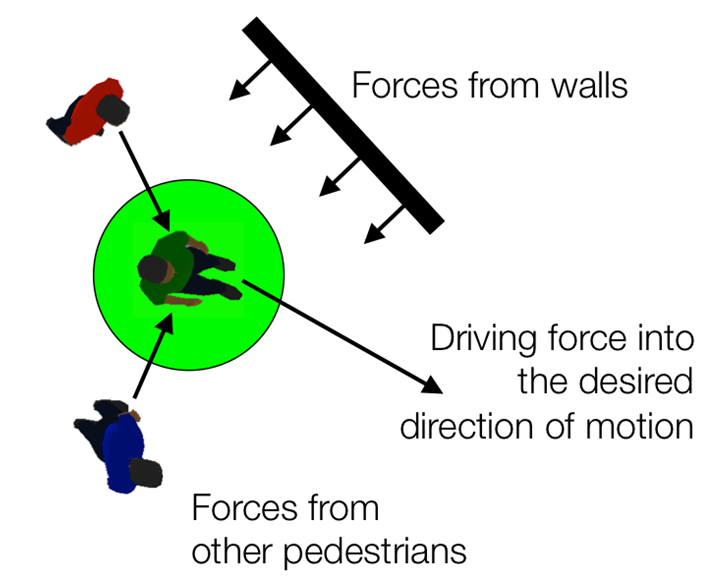
\includegraphics[width=0.40\linewidth]{Chapter1/social_force.png}
    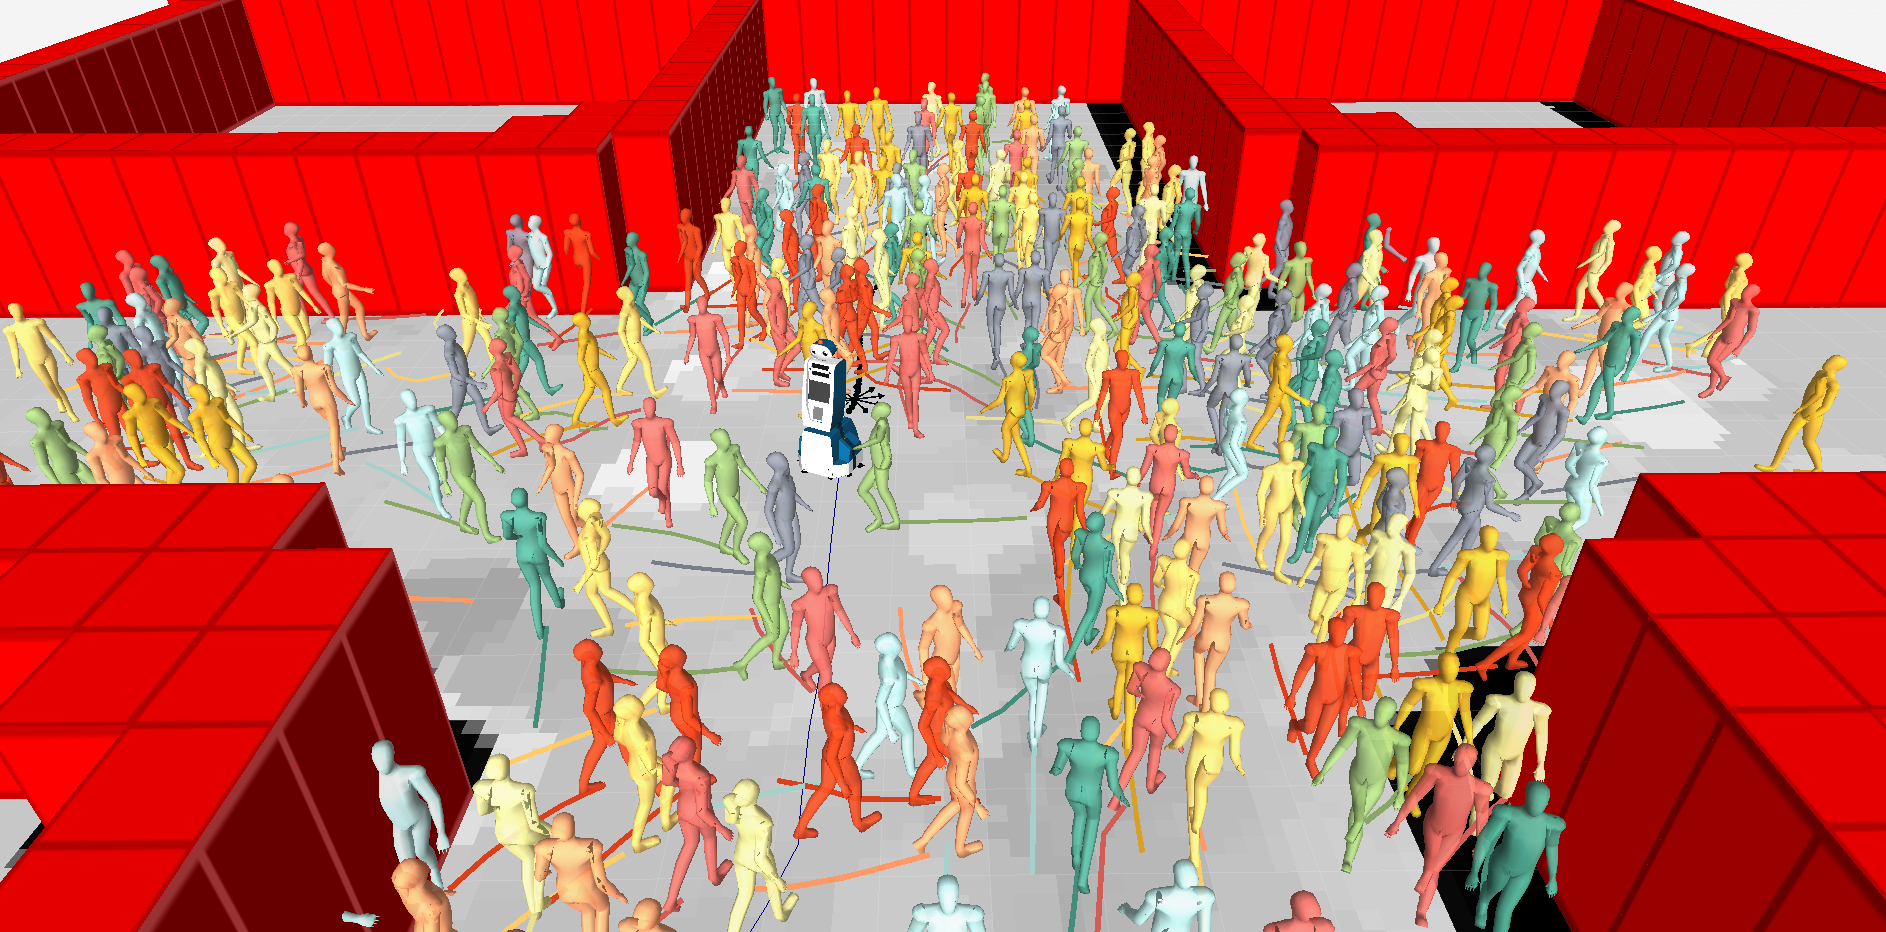
\includegraphics[width=0.54\linewidth]{Chapter1/crowd1.png}
    \caption{Social force model approximating pedestrian motion by a sum of forces.}
    \label{fig:social_force_model}
\end{figure}

Typical approaches involve reactive-only techniques such as social force models \cite{helbing1995social,chen_social_2018}. 
The social force model assumes that a sum of different forces can approximate pedestrians' acceleration, deceleration, and directional changes, each capturing a different desire or interaction effect. For instance, as depicted in figure \ref{fig:social_force_model}, one force corresponds to the acceleration towards the desired velocity of motion; second, repulsive forces reflect the agent keeping a certain distance from other agents and obstacles; third, attractive forces represent the goal and motivations of the agent. Eventually, using standard physics equations, the sum of these dynamic forces describes the agents' motion.
Such reactive models are easy to use and efficient for crowd simulations. Interestingly, in crowded or evacuation scenarios, social force models exhibit several so-called ``self-organization phenomena'' such as lane formation, zipper effect, intermittent flow, or turbulence.
Unfortunately, such a model can perform very poorly in intricate and non-crowded scenarios involving some decision-making. Thus, there was a lack of intelligent simulated agents to challenge effectively \acrshort{han} system.
A few recent works also propose simulating human agents endowed with some reasoning processes. However, I did not find the time to compare my contribution with theirs, and it remains an interesting possible future work. Nevertheless, this shows that this is a subject of interest. Some related works will be discussed in Chapter~\ref{chap:6}.
